\chapter{\label{sec:app:helicityangle}\KS helicity angle}

\minitoc

Figure \ref{helicitycut} shows that the MC distribution of the cosine of Ks helicity angle is asymmetric. Physically the Ks helicity angle is expected to follow a symmetric $cos^2\theta$ distribution, however the observed asymmetry in this variable, manifest in both data and MC, was found to be due to the momentum and transverse momentum cuts placed on the bachelor pion in the stripping line. Figure \ref{helictyasymmetry} illustrates this point.

\begin{figure}[h]
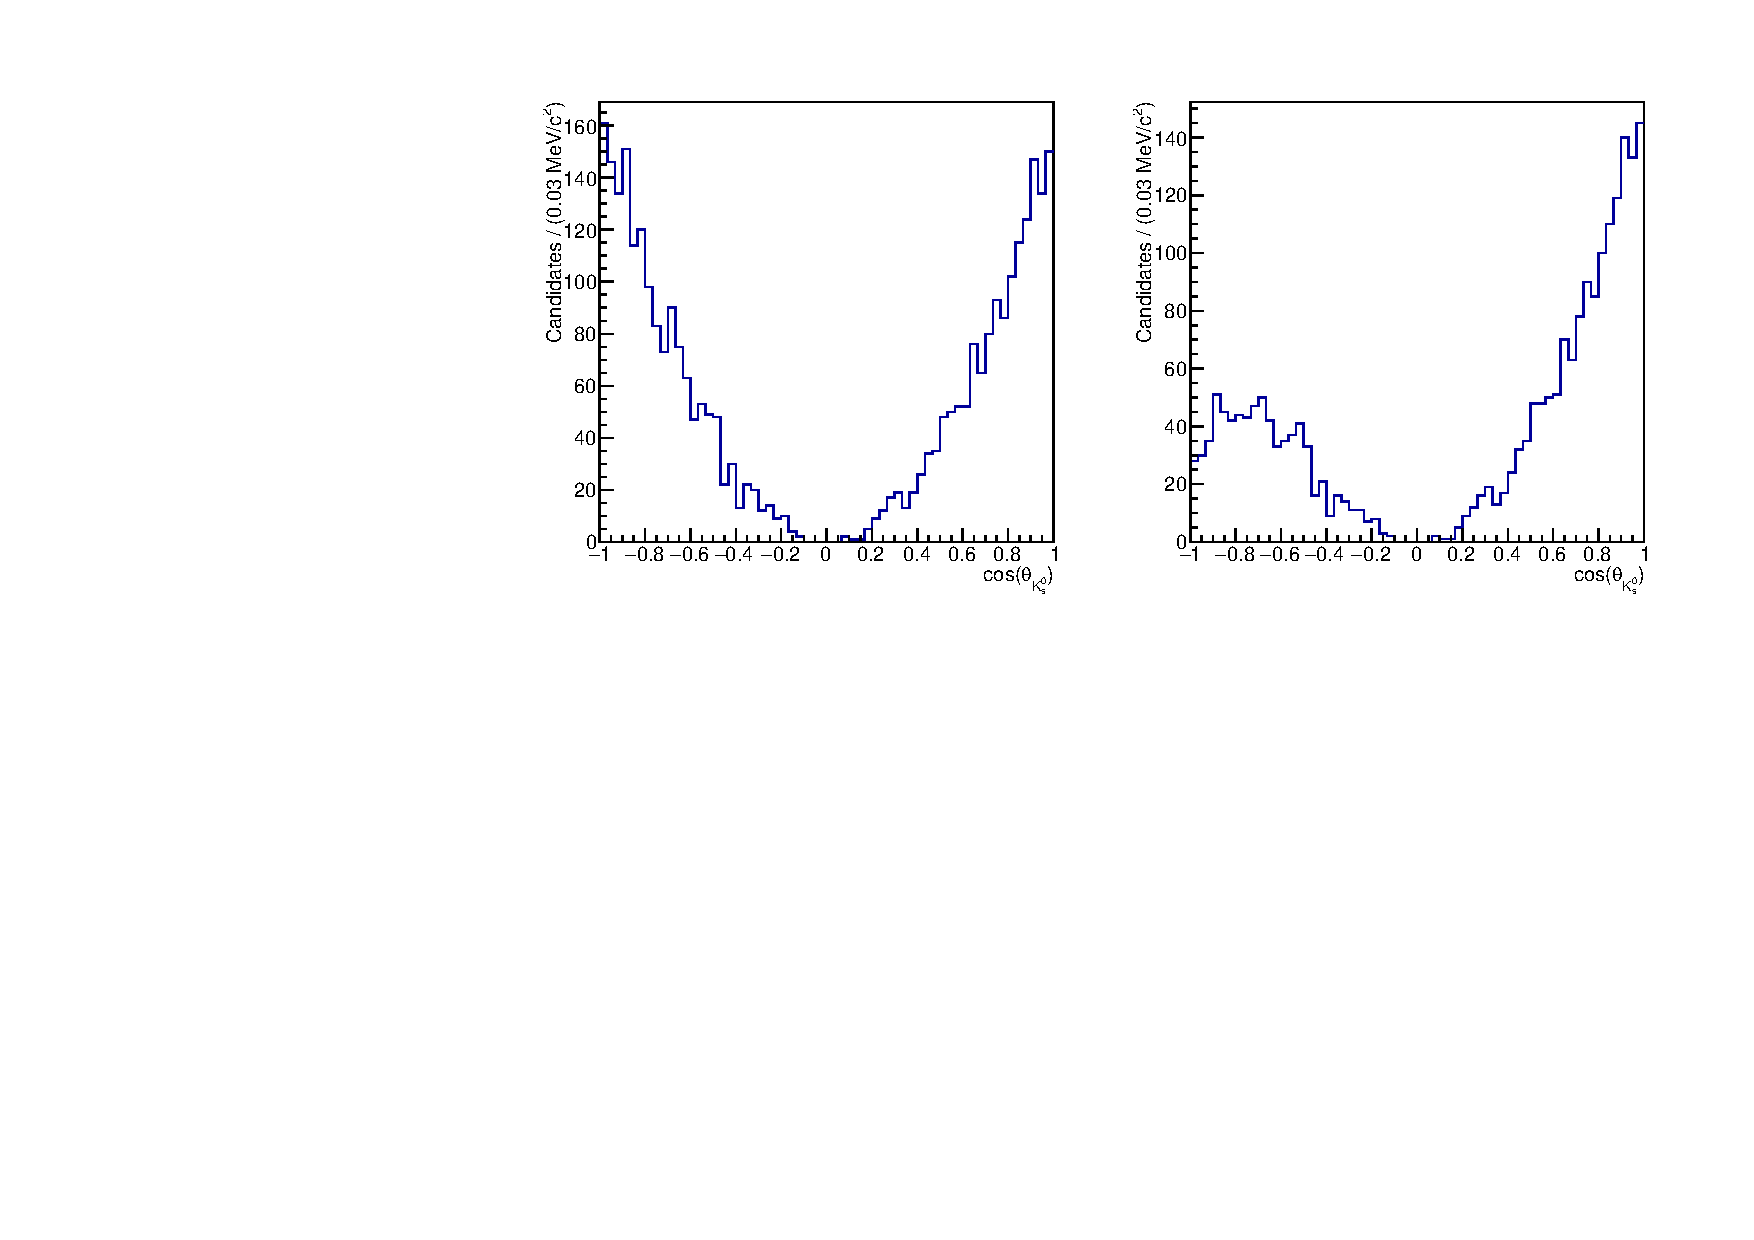
\includegraphics[width=\linewidth]{figures/helicityAngleAsymmetry.pdf}
\put(-360,150) {(a)}
\put(-150,150) {(b)}
\caption{\KS helicity angle MC distribution at generator level with (a) no cuts applied, and (b) bachelor $p > 2500$ MeV and bachelor $p_T > 250$ MeV, as in the stripping line}
\label{helictyasymmetry}
\end{figure}

\clearpage